\documentclass[11pt,a4paper]{article}
\usepackage[utf8]{inputenc}
\usepackage[czech]{babel}
\usepackage[IL2]{fontenc}
\usepackage{times}
\usepackage{amsmath}
\usepackage{amsfonts}
\usepackage{amssymb}
\usepackage{graphics}
\usepackage{fancyvrb}
\usepackage{multirow}
\usepackage{pdflscape}
\usepackage[ruled, czech, linesnumbered, noline, longend]{algorithm2e}
\usepackage[width=17.00cm, height=24.00cm, left=2.00cm, top=3.00cm]{geometry}
\author{Dominik Juriga}
\VerbatimFootnotes
\begin{document}
			\begin{titlepage}
				\begin{center} 
					\textsc{{\Huge Vysoké učení technické v~Brně} \\
					\vspace{0.6em}{\huge Fakulta informačních technologií}}\\
					\vspace{\stretch{0.382}}
					{\LARGE Typografie a publikování\,--\,3. projekt}\\
					\vspace{0.3em}
					{\Huge Tabulky a obrázky}
				\\
					\vspace{\stretch{0.618}}
				\end{center}
				{\Large 24. března 2019 \hfill Dominik Juriga}    
			\end{titlepage}
			\section{Úvodní strana}
			Název práce umístěte do zlatého řezu a nezapomeňte uvést dnešní datum a vaše jméno a přijmení.
			
			\section{Tabulky}
			Pro sázení tabulek můžeme použít buď prostředí\enspace\verb|tabbing|\enspace nebo prostředí \verb|tabular|.
		
			\subsection{Prostředí\enspace \texttt{tabbing}}
			Při použití\enspace \verb|tabbing|\enspace vypadá tabulka následovně: 
			
			\begin{tabbing}
				\textbf{Ovoce} \hspace{4em} \= \textbf{Cena} \hspace{1em} \=  \textbf{Množství}\\
				Jablka \> 25,90 \> 3 kg\\
				Hrušky \> 27,40 \> 2,5 kg\\
				Vodní melouny \> 35,-- \> 1 kus
			\end{tabbing} \vspace{1em}
			Toto prostředí se dá také použít pro sázení algoritmů, ovšem vhodnejší je použít prostředí\enspace\verb|algorithm|\enspace nebo \enspace\verb|algorithm2e|\enspace (viz sekce \ref{sec3}).
			
			\subsection{Prostředí\enspace \texttt{tabular}}
			Další možností, jak vytvořit tabulku, je použít prostředí \enspace \verb|tabular|. Tabulky pak budou vypadat takto\footnote{Kdyby byl problém s\enspace \verb|cline|, zkuste se podívat třeba sem:   http://www.abclinuxu.cz/tex/poradna/show/325037.}:
			\vspace{1em}
			\begin{table}[h]
				\catcode`\-=12 %cline fix
				\begin{center}	
					\begin{tabular}{| l | c | r |} \hline

						&\multicolumn{2}{c|}{\textbf{Cena}} \\ \cline{2-3}
						\textbf{Měna} & \textbf{nákup} & \textbf{prodej} \\ \hline
						EUR & 25,615 & 27,20\\
						GBP & 29,899 & 31,80\\
						USD & 22,571 & 25,51 \\ \hline
					\end{tabular}
					\caption{Tabulka kurzů k~dnešnímu dni}
					\label{kurzovylistok}
				\end{center}
			\end{table}
		\begin{table}[h]
			\centering
			\begin{tabular}{|c|c|}
				\hline
				\multicolumn{1}{|c|}{A} & $\neg$A \\ \hline
				\textbf{P}                       & N \\ \hline
				\textbf{O}                       & O~\\ \hline
				\textbf{X}                       & X \\ \hline
				\textbf{N}                       & P \\ \hline
			\end{tabular}
		\catcode`\-=12 %cline fix
		\begin{tabular}{|c|c|c|c|c|c|}
			\hline
			\multicolumn{2}{|c|}{\multirow{2}{*}{A $\wedge$ B}} & \multicolumn{4}{c|}{B} \\ \cline{3-6} 
			\multicolumn{2}{|c|}{}                   & \textbf{P}    & \textbf{O}   & \textbf{X}   & \textbf{N}   \\ \hline
			\multirow{4}{*}{A}          & \textbf{P}          & P    & O~& X   & N   \\ \cline{2-6} 
			& \textbf{O}          & O~& O~& X   & N   \\ \cline{2-6} 
			& \textbf{X}          & X    & N   & X   & N   \\ \cline{2-6} 
			& \textbf{N}          & N    & N   & N   & N   \\ \hline
		\end{tabular}
	\catcode`\-=12 %cline fix
	\begin{tabular}{|c|c|c|c|c|c|}
		\hline
		\multicolumn{2}{|c|}{\multirow{2}{*}{A $\vee$ B}} & \multicolumn{4}{c|}{B} \\ \cline{3-6} 
		\multicolumn{2}{|c|}{}                   & \textbf{P}    & \textbf{O}   & \textbf{X}   & \textbf{N}   \\ \hline
		\multirow{4}{*}{A}          & \textbf{P}          & P    & P   & P   & P   \\ \cline{2-6} 
		& \textbf{O}          & P    & O~& P   & O~\\ \cline{2-6} 
		& \textbf{X}          & P    & P   & X   & X   \\ \cline{2-6} 
		& \textbf{N}          & P    & O~& X   & N   \\ \hline
	\end{tabular}
	\catcode`\-=12 %cline fix
	\begin{tabular}{|c|c|c|c|c|c|}
		\hline
		\multicolumn{2}{|c|}{\multirow{2}{*}{A $\rightarrow$ B}} & \multicolumn{4}{c|}{B} \\ \cline{3-6} 
		\multicolumn{2}{|c|}{}                   & \textbf{P}    & \textbf{O}   & \textbf{X}   & \textbf{N}   \\ \hline
		\multirow{4}{*}{A}          & \textbf{P}          & P    & O~& X   & N   \\ \cline{2-6} 
		& \textbf{O}          & P    & O~& P   & O~\\ \cline{2-6} 
		& \textbf{X}          & P    & P   & X   & X   \\ \cline{2-6} 
		& \textbf{N}          & P    & P   & P   & P   \\ \hline
	\end{tabular}
\caption{Protože Kleeneho trojhodnotová logika už je \uv{zastaralá}, uvádíme si zde příklad čtyřhodnotové logiky}
\label{logika}
\end{table}\\ \pagebreak
		
			\section{Algoritmy}\label{sec3}
			Pokud budeme chtít vysázet algoritmus, můžeme použít prostředí \texttt{algorithm}\footnote{Pro nápovědu, jak zacházet s~prostředím \verb|algorithm|, můžeme zkusit tuhle stránku:\\ http://ftp.cstug.cz/pub/tex/CTAN/macros/latex/contrib/algorithms/algorithms.pdf.} nebo \texttt{algorithm2e}\footnote{Pro \enspace\verb|algorithm2e| zase tuhle: http://ftp.cstug.cz/pub/tex/CTAN/macros/latex/contrib/algorithm2e/doc/algorithm2e.pdf.}.\linebreak
			\noindent Příklad použití prostředí \verb|algorithm2e| viz Algoritmus \ref{alg}.\\
			
			\IncMargin{1.5em}
			\begin{algorithm}
				\caption{\textsc{FastSLAM}}
				\label{alg}
				
				\SetInd{1em}{1em}
				\SetAlgoNlRelativeSize{-1}
				\SetNlSty{}{}{:}
				\SetNlSkip{0.4em}
				
				\Indm
				\Indmm
				\KwIn{$ (X_{t - 1}, u_t, z_t) $}
				\KwOut{$ X_t $}
				\Indp\Indpp
				\BlankLine
				
				$ \overline{X_t} = X_t = 0 $ \\
				
				\For{$ k~= 1 \textrm{\emph{ to }} M $}{
					$ x_t^{[k]} = \emph{sample\_motion\_model}(u_t, x_{t - 1}^{[k]}) $ \\
					$ \omega_t^{[k]} = \emph{measurement\_model}(z_t, x_t^{[k]}, m_{t - 1}) $ \\
					$ m_t^{[k]} = updated\_occupancy\_grid(z_t, x_t^{[k]}, m_{t - 1}^{[k]}) $ \\
					$ \overline{X_t} = \overline{X_t} + \langle x_x^{[m]}, \omega_t^{[m]}  \rangle $ \\
				}
				
				\For{$ k~= 1 \textrm{\emph{ to }} M $}{
					draw $ i $ with probability $ \approx \omega_t^{[i]} $ \\
					add $ \langle x_x^{[k]}, m_t^{[k]} \rangle \textrm{ to } X_t $ \\
				}
				
				\Return{$ X_t $}
			\end{algorithm}
		\DecMargin{1.5em}
		
		\section{Obrázky}
		Do našich článků můžeme samozřejmě vkládat obrázky. Pokud je obrázkem fotografie, můžeme klidně použít bitmapový soubor. Pokud by to ale mělo být nejaké schéma nebo něco podobného, je dobrým zvykem takovýto obrázek vytvořit vektorově.
		
		\begin{figure}[h]
			\centering
			\scalebox{0.4}{
				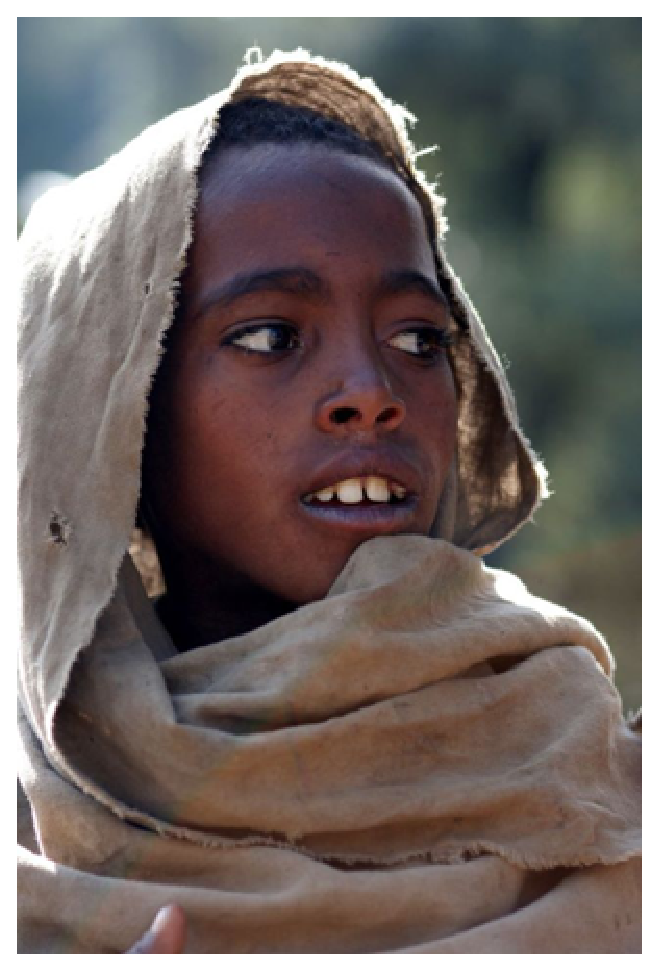
\includegraphics{etiopan.eps}
				\reflectbox{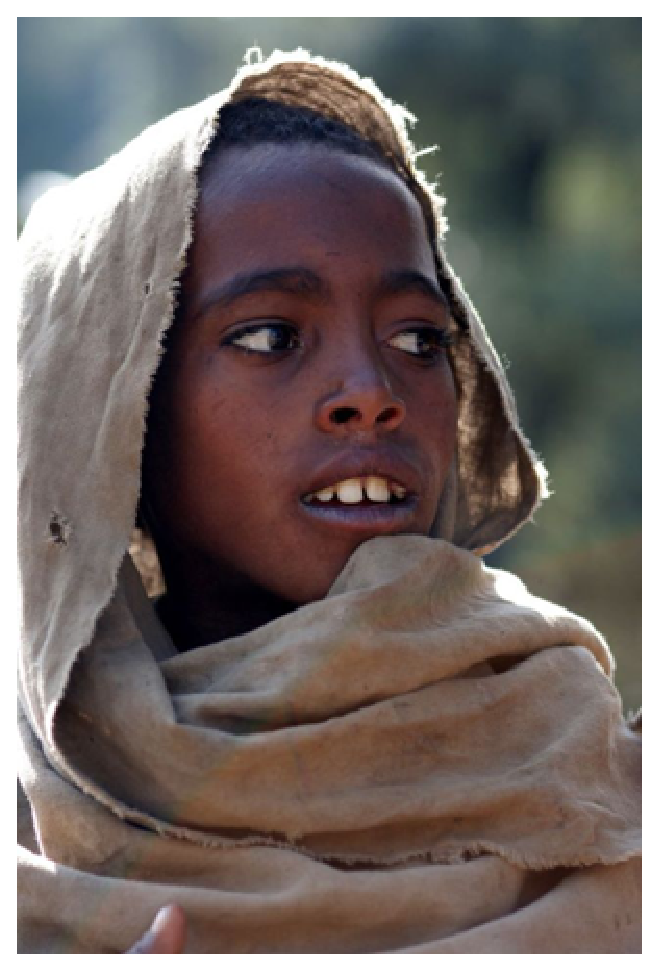
\includegraphics{etiopan.eps}}
			}
			\caption{Malý Etiopánek a~jeho bratříček}
			\label{eti}
		\end{figure}
	\newpage
	
	Rozdíl mezi vektorovým\,\dots

\begin{figure}[h]
	\scalebox{0.4}{
\includegraphics{oniisan.eps}}
	\centering
	\caption{Vektorový obrázek}
	\label{vec}
\end{figure}
\bigskip
\noindent \dots\,a~bitmapovým obrázkem

\begin{figure}[h]
	\scalebox{0.6}{
\includegraphics{oniisan2.eps}}
	\centering
	\caption{Bitmapový obrázek}
	\label{bitmap}
\end{figure}
\bigskip
\noindent se projeví například při zvětšení.

Odkazy (nejen ty) na obrázky~\ref{eti},~\ref{vec} a~\ref{bitmap}, na
tabulky~\ref{kurzovylistok} a~\ref{logika}~a také na algoritmus~\ref{alg} jsou
udělány pomocí křížových odkazů. Pak je ovšem potřeba zdrojový soubor přeložit dvakrát.
	
	Vektorové obrázky lze vytvořit i~přímo v~{\LaTeX}u, například pomocí prostředí\texttt{ picture.}
	
	\begin{landscape}
		\begin{figure}[h]
			\setlength{\unitlength}{1mm}
			\centering
			\begin{picture}(200, 110)
			\linethickness{1pt}
			\put(0, 0){\framebox(200, 100){}}
			
			\linethickness{0.4mm}
			
			\put(10, 10){\line(1,0){30}} %podlaha garaz
			\put(13, 30){\line(1,0){24}} %brana top garaz
			\put(13, 10){\line(0,0){20}} %brana lava garaz
			\put(37, 10){\line(0,0){20}} %brana prava garaz
			\put(10, 10){\line(0,0){20}} %lava stena garaz
			\put(40, 10){\line(0,0){20}} %prava stena garaz
			\put(10, 30){\line(1,1){15}} %lava strecha garaz
			\put(25, 45){\line(1,-1){15}} %prava strecha garaz
			
			\put(50, 10){\line(1,0){120}} %dom podlaha
			\put(50, 10){\line(0,0){40}} %dom lava stena
			\put(170, 10){\line(0,0){40}} %dom prava stena
			\put(50, 50){\line(1,1){20}} %dom lava polka lava strecha
			\put(70, 70){\line(1,-1){20}} %dom lava polka prava strecha
			\put(130, 50){\line(1,1){20}} %dom prava polka lava strecha
			\put(150, 70){\line(1,-1){20}} %dom prava polka prava strecha
			\put(90, 50){\line(1,0){40}} %dom stred spoj
			\put(100, 10){\line(0,0){15}} %dom dvere lava strana
			\put(110, 10){\line(0,0){15}} %dom dvere stredna strana
			\put(120, 10){\line(0,0){15}} %dom dvere prava strana
			\put(100, 25){\line(1,0){20}} %dom dvere vrchna strana
			
			\put(60, 35){\line(0,0){10}} %dom lave okno lava strana
			\put(70, 35){\line(0,0){10}} %dom lave okno stredna strana
			\put(80, 35){\line(0,0){10}} %dom lave okno prava strana
			\put(60, 35){\line(1,0){20}} %dom lave okno vrchna strana
			\put(60, 45){\line(1,0){20}} %dom lave okno vrchna strana
			
			\put(140, 35){\line(0,0){10}} %dom prave okno lava strana
			\put(150, 35){\line(0,0){10}} %dom prave okno stredna strana
			\put(160, 35){\line(0,0){10}} %dom prave okno prava strana
			\put(140, 35){\line(1,0){20}} %dom prave okno vrchna strana
			\put(140, 45){\line(1,0){20}} %dom prave okno vrchna strana
			
			\put(97, 35){\line(0,0){10}} %dom stredne okno lava strana
			\put(102, 35){\line(0,0){10}} %dom stredne okno prava strana
			\put(97, 35){\line(1,0){5}} %dom stredne okno vrchna strana
			\put(97, 45){\line(1,0){5}} %dom stredne okno vrchna strana
			
			\put(104, 35){\line(0,0){10}} %dom stredne okno lava strana
			\put(109, 35){\line(0,0){10}} %dom stredne okno prava strana
			\put(104, 35){\line(1,0){5}} %dom stredne okno vrchna strana
			\put(104, 45){\line(1,0){5}} %dom stredne okno vrchna strana
			
			\put(111, 35){\line(0,0){10}} %dom stredne okno lava strana
			\put(116, 35){\line(0,0){10}} %dom stredne okno prava strana
			\put(111, 35){\line(1,0){5}} %dom stredne okno vrchna strana
			\put(111, 45){\line(1,0){5}} %dom stredne okno vrchna strana
			
			\put(118, 35){\line(0,0){10}} %dom stredne okno lava strana
			\put(123, 35){\line(0,0){10}} %dom stredne okno prava strana
			\put(118, 35){\line(1,0){5}} %dom stredne okno vrchna strana
			\put(118, 45){\line(1,0){5}} %dom stredne okno vrchna strana
			
			
			
			
			\put(45, 80){\circle{20}}
			\end{picture}
			\caption{Vektorový obrázek moderního bydlení vhodného pro 21. století.}
		\end{figure}
	\end{landscape}
	
\end{document}